\documentclass{article}
\usepackage{graphicx}
\usepackage{titletoc}
\usepackage{titlesec}
\usepackage{geometry} 
\usepackage{fontspec, xunicode, xltxtra}
\usepackage{float}
\usepackage{cite}
\usepackage{amsmath}
\usepackage{listings}
\usepackage{titletoc}
\usepackage{booktabs}

\geometry{left=3cm,right=3cm,top=3cm,bottom=3cm}
\DeclareMathOperator*{\argmin}{argmin}
\DeclareMathOperator*{\argmax}{argmax}
\DeclareMathOperator*{\logit}{logit}
\DeclareMathOperator*{\var}{var}
\DeclareMathOperator*{\cov}{cov}
\DeclareMathOperator*{\expec}{E}
\DeclareMathOperator*{\deriv}{d}
\DeclareMathOperator*{\const}{constant}

\begin{document}
\title{\textsf{Homework 6 for Bayesian Data Analysis}}
\author{Fan JIN\quad (2015011506)}
\maketitle

\section*{Question 10.4a}
{
    Let the identity function $I$ indicate whether a sample $x$ is accepted or not. It follows that 
    $$p(I=1) = \int{ p(I=1 | x) g(x) \deriv{x} }$$
    $$= \int{ \frac{f(x)}{c g(x)} g(x) \deriv{x} }$$
    $$= \int{ \frac{f(x)}{c} \deriv{x} } = \frac{1}{c}.$$

    Then, we have 
    $$p(x | I=1) = p(x, I=1) / p(I=1)$$
    $$= g(x) \frac{f(x)}{c g(x)} / \frac{1}{c} = f(x).$$
}

\section*{Question 10.4b}
{
    To make the integral above valid, it requires 1) the denominator $g(x)>0$ for any $x$ that satisfies $f(x)>0$, and 2) the probability $f(x) / c g(x) \leq 1$ for any $x$. These two requirements cannot be met unless $f(x)/g(x)$ is bounded.
}

\section*{Question 10.6}
{
    Without loss of generality, suppose the posterior distribution is normal $N(0, 3)$, which matches, in mode and curvature (variance), to the standard $t_3$ distribution. 
    \begin{table}[H]
        \centering
        \caption{Estimated posterior expectation and variance}
        \begin{tabular}{@{}clc@{}clc@{}}
        \toprule
        sample size & \multicolumn{1}{c}{E (estimated)} & \multicolumn{1}{c}{E (true)} & \multicolumn{1}{c}{Var (estimated)} & \multicolumn{1}{c}{Var (true)}  \\ \midrule
        100 & 0.076218 & 0 & 3.043008 & 3   \\ 
        10000 & -0.035262 & 0 & 3.051913 & 3  \\ \bottomrule
        \end{tabular}
    \end{table}
    The estimation is accurate even for a small sample size ($S=100$).
    Some importance weights are extremely small, but no weights are extremely large. This implies well behaved importance weights.
    \begin{figure}[H]
        \centering
        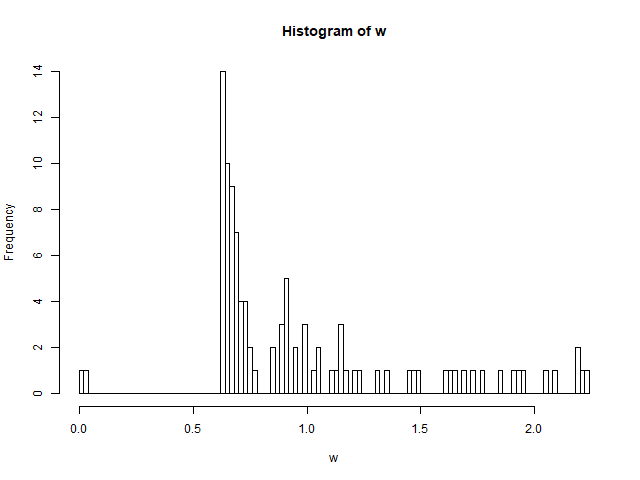
\includegraphics[width = 0.6\linewidth]{1_weight_100.png}
        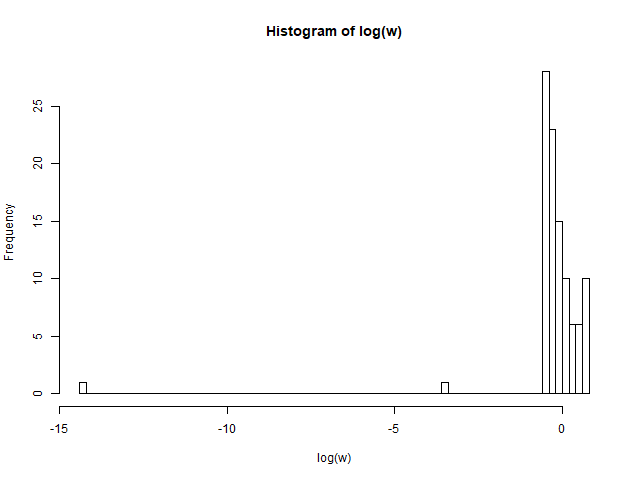
\includegraphics[width = 0.6\linewidth]{1_log_weight_100.png}
        \caption{Sample size = 100}
    \end{figure}
    \begin{figure}[H]
        \centering
        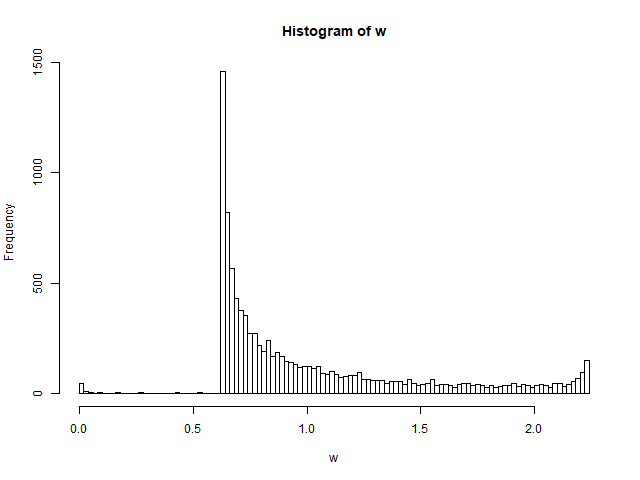
\includegraphics[width = 0.6\linewidth]{1_weight_10000.png}
        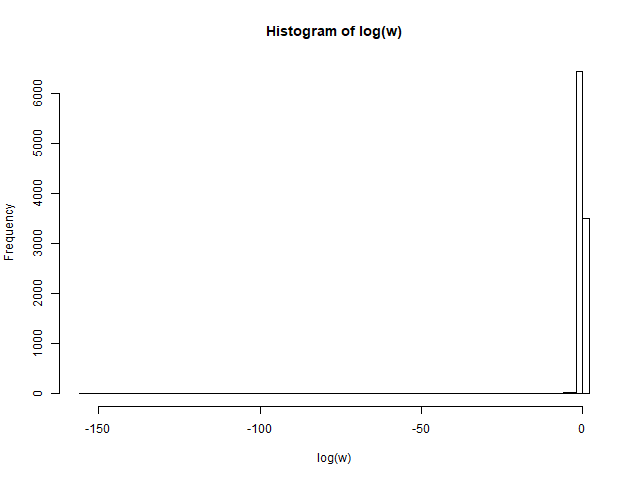
\includegraphics[width = 0.6\linewidth]{1_log_weight_10000.png}
        \caption{Sample size = 10000}
    \end{figure}

}

\section*{Question 10.7}
{
    Without loss of generality, suppose the posterior distribution is standard $t_3$, which matches, in mode and curvature (variance), to the normal $N(0, 3)$ distribution. 
    \begin{table}[H]
        \centering
        \caption{Estimated posterior expectation and variance}
        \begin{tabular}{@{}clc@{}clc@{}}
        \toprule
        sample size & \multicolumn{1}{c}{E (estimated)} & \multicolumn{1}{c}{E (true)} & \multicolumn{1}{c}{Var (estimated)} & \multicolumn{1}{c}{Var (true)}  \\ \midrule
        100 & 0.084248 & 0 & 1.648969 & 1   \\ 
        10000 & -0.008052 & 0 & 2.193678 & 1  \\ \bottomrule
        \end{tabular}
    \end{table}
    The estimation is not accurate even for a large sample size ($S=10000$).
    Some importance weights are extremely large, especially for large sample size. This implies the importance weights are too variate, and therefore, explains why our estimation is even worse when we have larger sample size: 
    
    Since the $t$ distribution has heavier tails than the normal distribution does, we can hardly draw a sample at the tail from simulation based on normal distribution. With a large sample size, it is more likely that such a tail sample is drawn, leading to a large importance weight. This would increase the variance of our estimation, as the weights are not so uniform. According to the textbook, the estimation is sensitive to an outlier of extremely large importance weight (when we try to estimate heavy tailed distribution with a light tailed one), while it is not when we try to estimate in the reversed way.
    \begin{figure}[H]
        \centering
        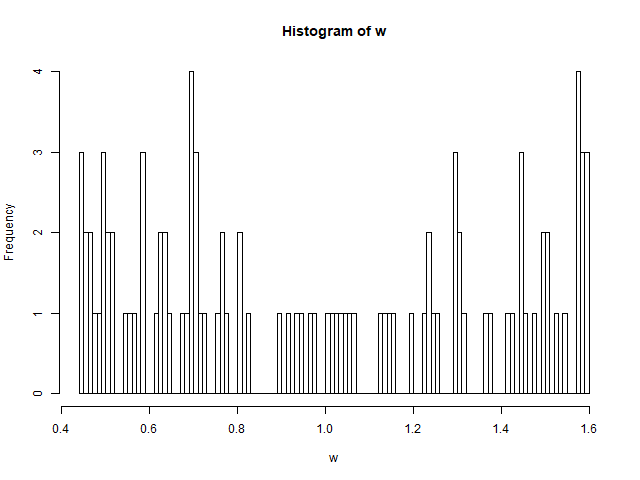
\includegraphics[width = 0.6\linewidth]{2_weight_100.png}
        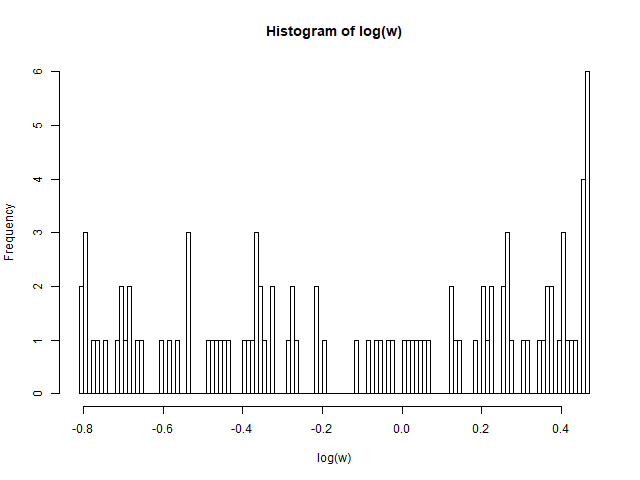
\includegraphics[width = 0.6\linewidth]{2_log_weight_100.png}
        \caption{Sample size = 100}
    \end{figure}
    \begin{figure}[H]
        \centering
        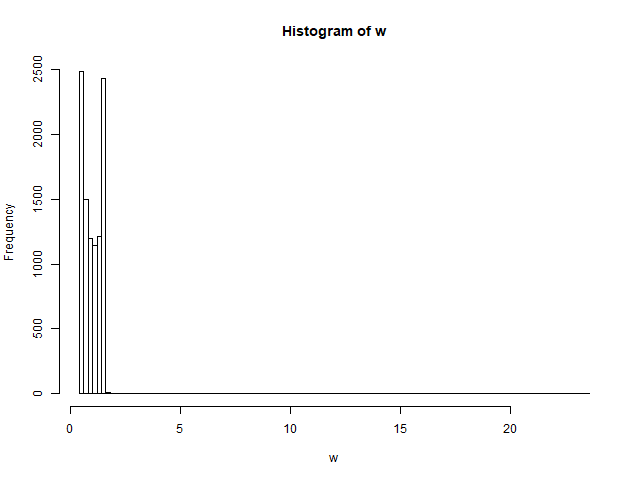
\includegraphics[width = 0.6\linewidth]{2_weight_10000.png}
        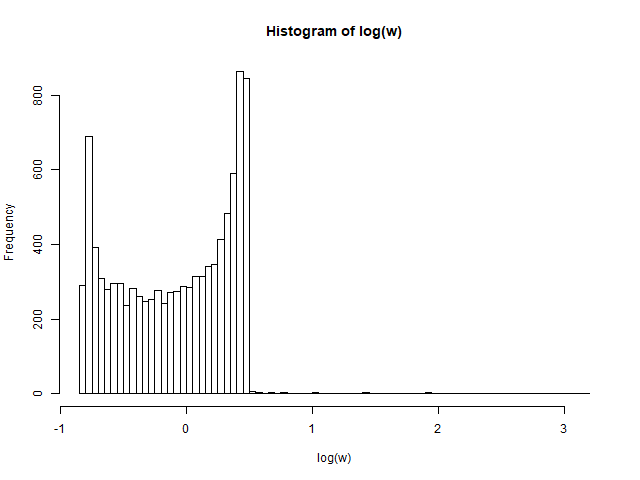
\includegraphics[width = 0.6\linewidth]{2_log_weight_10000.png}
        \caption{Sample size = 10000}
    \end{figure}
}

\section*{Source Code in R}
{
    \begin{lstlisting}[language=R]
        set.seed(2018)

        weight <- function(x) {
          return (dnorm(x, sd = sqrt(3)) / dt(x, 3))
        }
        
        for (S in c(100, 10000)) {
          t = rt(S, 3)
          w = unlist(lapply(t, weight))
          
          png(sprintf("1_weight_%d.png", S), width = 640, height = 480)
          hist(w, breaks = 100)
          dev.off()
          
          png(sprintf("1_log_weight_%d.png", S), width = 640, height = 480)
          hist(log(w), breaks = 100)
          dev.off()
          
          first.order = mean(t * w) / mean(w)
          second.order = mean(t^2 * w) / mean(w)
          
          expectation = first.order
          variance = second.order - first.order^2
          
          print(sprintf("1: size = %d, expectation = %f, 
                        variance = %f", S, expectation, variance))
        }
        
        weight <- function(x) {
          return (dt(x, 3) / dnorm(x, sd = sqrt(3)))
        }
        
        for (S in c(100, 10000)) {
          n = rnorm(S, sd = sqrt(3))
          w = unlist(lapply(n, weight))
          
          png(sprintf("2_weight_%d.png", S), width = 640, height = 480)
          hist(w, breaks = 100)
          dev.off()
          
          png(sprintf("2_log_weight_%d.png", S), width = 640, height = 480)
          hist(log(w), breaks = 100)
          dev.off()
          
          first.order = mean(n * w) / mean(w)
          second.order = mean(n^2 * w) / mean(w)
          
          expectation = first.order
          variance = second.order - first.order^2
          
          print(sprintf("2: size = %d, expectation = %f, 
                        variance = %f", S, expectation, variance))
        }
    \end{lstlisting}
}

\clearpage
\end{document}
